% !TeX spellcheck = en_US
\documentclass[a4paper]{article}
\usepackage{graphicx}
\usepackage{geometry}
\usepackage{enumerate}
\geometry{left = 2.0 cm, right = 2.0cm}
\begin{document}
\title{Design Report of 16 Taps Programmable FIR Filter}
\author{KANG Jian \qquad ID:20440622}
\date{}
\maketitle
\section{Design Methodology of Programmable 16 taps FIR Filter}
There are some essential requirements in the document as below:
\begin{enumerate}[1)]
\item The number of taps can be controlled by users.
\item Both coefficient and data are fixed point 8-bits 2’s complement numbers.
\item Two output signal to indicate overflow and direction.
\item The chip interface with outside using handshake signal.
\item Just four MAC units can be used in the design.
\end{enumerate}
According these requirements, The filter can be divided into four parts which are control module, Multiply and Accumulate module(MAC), Configuration module and Top module. MAC is arithmetic part which multiplies the coefficient and data and accumulate them together. Configuration module is responsible to the initial coefficients and taps number. When the port \emph{configuration} is pulled up. This module could also modify the value of coefficients and taps number. Control module is responsible for detect the input signal and decide the working state. It give enable signals to others modules to make them work as order. Top module instantiates other modules and creates input and output ports. Figure \ref{fig:16_FIR} shows the whole structure of this design. 
\begin{figure}[htb]
\centering
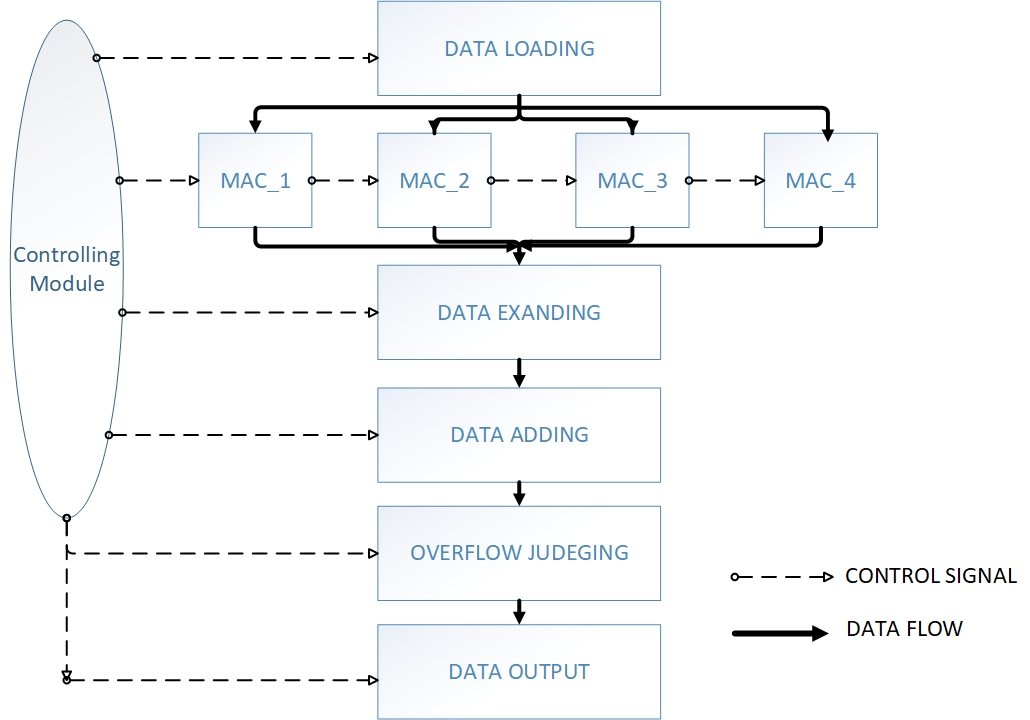
\includegraphics[scale=0.5]{pic/FIR_structure}
\caption{Structure of Programmable FIR Filter}
\label{fig:16_FIR}
\end{figure}
In \ref{subsec1_1} and \ref{subsec1_2}, MAC unit and Controlling module will be introduced. And other modules will also be introduce in \ref{subsec1_3}. The \ref{sec_2} will introduce the test-bench and simulation. \ref{sec_3} is about constrain and synthesis. \ref{sec_4} is the summary and places that can be improved.
\subsection{MAC Design}\label{subsec1_1}
The maximum taps is 16 and we could only use 4 MAC units. So each unit needs to do 4 times multiplication and accumulation. This core of this unit is a counter. and there's also a combinational logic in this design which is responsible for data expand, multiplication and accumulation. When \emph{enable} of this module is pulled up. The counter will work. it provides one coefficient and one data to the combinational logic each time and receives the accumulation value from combinational logic. when the counter is 4, MAC will export the final result and pulls up done signal to indicate that it has completed its work. The handshake mechanism is used in this module. At the same time, MAC can be disabled according the taps number to save power. Figure \ref{fig:MAC} shows the structure of this module. 
\begin{figure}[htb]
\centering
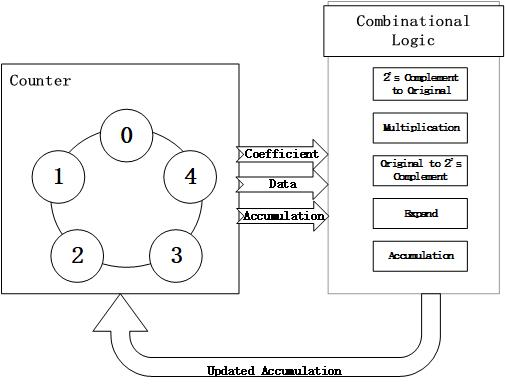
\includegraphics[scale=0.6]{pic/MAC_design}
\caption{Multiplication and Accumulation Module}
\label{fig:MAC}
\end{figure}

One point should be cared which is the fix point number. The coefficient and input data is all fractional and 2's complement number. The numbers are firstly transfered to original number to do multiplication and choose the 8 bits most significant part as the result. Then the result is transfered to 2's complement number for the accumulation. But there are totally four 8 bits number will be added together. Overflow may be happen. But overflow detect should be done inside MAC units because there are four MACs in the filter.Overflow figures may cancel each other. Increase the integer part can solve this problem. The result is expanded from 8 bits like $x.xxxxxxx$ to 10 bits like $xxx.xxxxxxx$. The first bit is sign bit. So the result of MAC is 10 bits.
\subsection{Controlling Module Design}\label{subsec1_2}
MAC unit is arithmetic part and controlling module is control part as its name. Actually it is a classical Finial State Mechine. there are eight states being defined. When the \emph{enable} and \emph{configuration} are both pulled down. This system is in IDLE state. all modules controlled by it are disabled. When \emph{enable} are pulled up. The state is changed to LOAD and \emph{load\_enable} signal will be pulled up. Then the state is changed to CALCU and controlling module will pull up \emph{MAC\_enable} signal according the taps number to save power. The controlling module will wait for \emph{mac\_done} signal. After \emph{mac\_done} signal is pulled up. The state is changed to EXPAND. \emph{expand\_enable} will be pulled up. Then the state is changed to ADD. \emph{add\_enable} is pulled up. Then state becomes JUDGE. \emph{JUDGE} is pulled up. Then the state becomes DONE. \emph{done} is pulled up. If \emph{configuration} is always low. the state will never change to CONFIG. But once \emph{configuration} is pulled up. The state will change to configuration at one. In this state, input data is used to configure coefficient and taps number. After configuration, just pull down \emph{configuration} and state will be changed to IDLE and wait for \emph{enable} to processing data again. The state transfer can be shown like Figure \ref{fig:CONTROL}
\begin{figure}[htb]
	\centering
	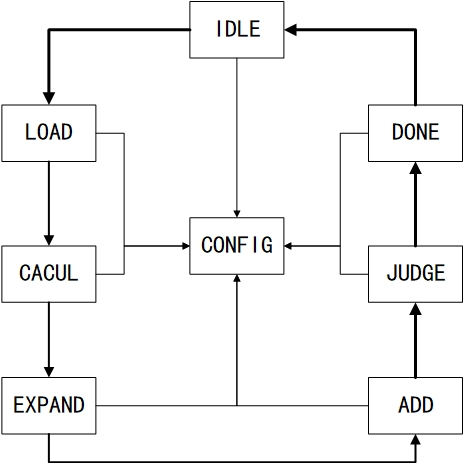
\includegraphics[scale=0.6]{pic/control}
	\caption{FIR Controlling Module}
	\label{fig:CONTROL}
\end{figure}

Each state control a module to work or not. In IDLE state, no module works. In LOAD state, load module works to load data. In CALCU state, MAC work to calculation multiplication and accumulation result. In EXPAND state, the 10 bits result like $xxx.xxxxxxx$ is expanded to 12 bits like $xxxxx.xxxxxxx$ to avoid overflow. In ADD state, the expanded result from all four MACs will be added together. In JUDGE state, the 12 bits result will be catted to 8 bits like $x.xxxxxxx$ again. If the result is large than 1. The output will be $0.1111111$ and the overflow flag will be $01$. If the result is smaller than -1, the output will be $1.0000000$ and overflow flag will be $10$. The MAC is introduced before. How about loading,judging and configuration? \ref{subsec1_3} introduce the details about that.

\subsection{Other Module Design}\label{subsec1_3}
The system store coefficients and data in the registers. How to load the data into the registers. Because of features of the FIR filter. one data will be updated to the registers. So the structure of the register could be shown like Figure \ref{fig:load}. It is like a simple FIFO. If the taps number is reduced, we just configure the coefficient as zero. So the left value will not influence the final result.
\begin{figure}[htb]
	\centering
	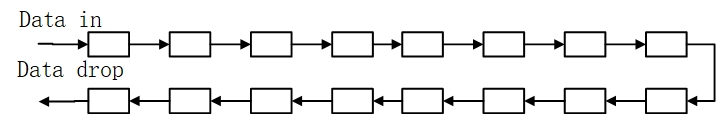
\includegraphics[scale=0.6]{pic/load}
	\caption{Data Load}
	\label{fig:load}
\end{figure}

How to judge the overflow? The sum of 4 MACs is a 12 bit number like $xxxxx.xxxxxxx$, The first bit is sign bit. If the first bit 1, it means that this number is negative. If any other bits of integer part is 0, it means the result is less than -1 which means there exists negative overflow. If the first bit is 0, it means the result is positive. If any other bis of integer part is 1, it means the result is larger than 1. There exists positive overflow. It is not so difficult. But it needs the inner result has 12 bits.

The project requires the filter is programmable. The design draft mentioned that IIC interface. But the configuration speed is slow and the operation is difficult. So, final design reuses the data input interface to configure the taps number and coefficients. In the configuration state, the data received from \emph{data\_in} is not used for data. When the \emph{config\_data\_enable} is high, the module get data from \emph{data\_in} port and configure taps number, h1 to h15 as order.  It is very easy to use and the speed is faster than IIC interface. 
\section{Time constrain and Post-Synthesis Simulation Result} 











\end{document}